\documentclass[hyperref,UTF8,titlepage]{ctexart}
\usepackage[a4paper]{geometry}
\usepackage{amsmath}
%\usepackage{MnSymbol}
\usepackage{bm}
\usepackage{siunitx}
\usepackage{fancyhdr}
\usepackage{float}
\usepackage[]{graphicx}
%\usepackage{pifont} % this is to provide macro \ding in line 12
%
%% \num{10e2}
%% \mmHg
%% \SI{4}{\milli\meter}
%% \gg  % instead of $>\!\!>$
%
%
%%% For footnote style
%\usepackage[perpage]{footmisc}
%\renewcommand\thefootnote{\ding{\numexpr171+\value{footnote}}}

\pagestyle{fancy}
%\geometry{a4paper, bottom=4cm}
%\graphicspath{{}}
\bibliographystyle{plain}

\hypersetup{
	colorlinks=false,
	pdftitle={},
	pdfauthor={Z. Y. Liu}}

\newcommand{\me}{\mathrm{e}}
\newcommand{\mi}{\mathrm{i}}
\newcommand{\diff}{\,\mathrm{d}}
\newcommand{\mRe}{\mathit{Re}}
%\newcommand{\mSt}{\mathit{St}}
%\newcommand{\mRo}{\mathit{Ro}}
%\newcommand{\Karman }{K\'arm\'an}

\title{重叠网格的有限体积法}
\author{刘泽宇}
\date{\today}

\begin{document}
\maketitle

\section{微分和积分形式的控制方程}

\subsection{任意维数的情形}
\label{sec:1.1}
对于物理量$\phi$的微分形式的控制方程为:
\begin{equation}
  \frac{\partial(\rho\phi)}{\partial t} = -\nabla\cdot(\rho\bm{v}\phi)+
  \nabla\cdot(\Gamma\nabla\phi)+S_\phi
  \label{eq:0}
\end{equation}
其中, $S_\phi$是源项, $\Gamma$是扩散系数.
该方程中, 令$\phi=1$得到质量方程, 令$\phi=u$则得到$x$方向
的动量方程. 构造有限体积法时使用方程(\ref{eq:0})对应的积分形式:
\begin{equation}\label{eq:00}
\frac{\partial}{\partial t}\int_V\rho\phi\diff V = -\int_{\partial V}\bm n\cdot(\rho\bm v\phi)\diff S +
\int_{\partial V} \bm n\cdot (\Gamma\nabla\phi)\diff S +\int_V S_\phi \diff V
\end{equation}
当$V$是以点$P$为中心的网格单元时, 上述方程可以进一步写成:
\begin{align}
  \frac{\diff}{\diff t}\left(\rho\phi_PV\right) 
  & = -\sum_e(\rho v_n\phi A)_e+\sum_e\Gamma(\bm n\cdot\nabla\phi)_e \label{eq:10} \\
  & = -\sum_eF_e\phi_e+\sum_e D_e(\phi_E-\phi_P)  \label{eq:11}\\ 
  & = -\sum_eJ_e \label{eq:12}
\end{align}
上述方程是有限体积法数值格式的理论基础, 若将$\phi_P$视为单元内物理量$\phi$的平均值, 那么上述离散方程仍然是
基本积分控制方程(\ref{eq:00})的等价方程. 单元体积的离散方程(\ref{eq:10})中的右边可以写成对流项和扩散项的和
如方程(\ref{eq:11})中所示, 有限体积法数值格式的构造的核心问题就是分别给出对流项和扩散项. 根据扩散项的物理性质,
梯度项$\nabla\phi$所对应的数值格式应该在整个网格上具有各向同性, 因此应该使用中心差分的格式对其进行离散. 而对于
对流项的离散则有多种方法, 详细内容在第~\ref{sec:scheme} 节中叙述.

\subsection{一维情形及线性Burgers方程}
\label{sec:1.2}
Navier-Stokes 方程在一维情形中, 质量方程退化消失, 动量方程就是Burgers方程:
\begin{equation}
  \label{eq:burgers}
  u_t+uu_x=\nu u_{xx}
\end{equation}
方程(\ref{eq:burgers})是非线性的, 虽有解析解, 但解的形式是隐式的, 较为复杂, 其简化的形式是将非线性项消除, 得到
线性化 Burgers 方程:
\begin{equation}
  \label{eq:lin-burgers}
  u_t+cu_x=\nu u_{xx}
\end{equation}
线性化Burgers方程的解析形式可以较为容易地得出, 对于边值问题:
\begin{equation*}
  \begin{cases}
    u_t+cu_x=\nu u_{xx} \\
    0<x<L\quad t\leq 0 \\
    u(0, t) = u_0 \quad u(L, t) = 0
  \end{cases}
\end{equation*}
其稳态的解析解可以写成用Reynold数$R=cL/\nu$表示的形式:
\begin{equation}
  \label{eq:ana-solution}
  u(x) = u_0\frac{1-\exp(R(x/L-1))}{1-\exp(-R)}
\end{equation}
对于$u_0=1$, $c=1$, $L=1$, $\nu=0.1$的情况, 可以画出上述解析解:
\begin{figure}[H]
  \centering
  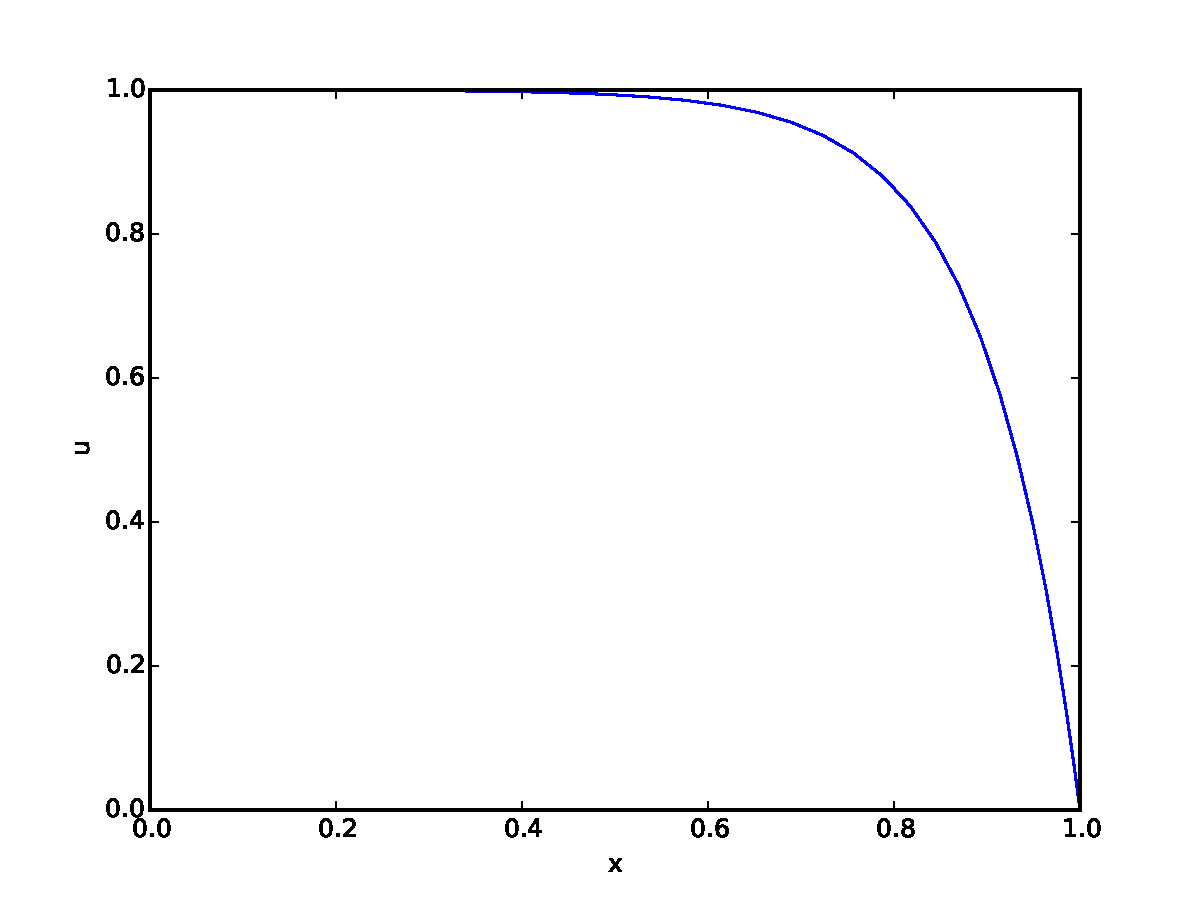
\includegraphics[width=0.7\textwidth]{exact.pdf}
  \caption{Burgers方程稳态解析解}
  \label{fig:ana-solution}
\end{figure}
图~\ref{fig:ana-solution} 和公式(\ref{eq:ana-solution})中的解析解既是数值格式优劣对比的标准, 
也是推导数值格式的重要辅助工具. 如果将计算的Reynold数设定得较大, 即采用很小的$\nu$容易导致解曲线
非常陡峭, 即出现激波解, 这时数值格式容易发散, 数值解和精确解的比较也比较困难, 因此将雷诺数设定为
$\mRe=1/\nu=10$.


\section{数值格式的构造}
\label{sec:scheme}

\subsection{经典有限体积法数值格式的构造}
\label{sec:scheme-classical}
根据方程(\ref{eq:11})(\ref{eq:12})可以得到:
\begin{equation}
  \label{eq:flux}
  J_e=F_e\phi_e-\frac{\Gamma A}{L}\frac{\partial\phi}{\partial x/L}
     =D_e\left(P_e\phi_e-\frac{\partial\phi}{\partial x/L}\right)
\end{equation}
方程(\ref{eq:flux})中引入了Peclet数$P_e$, 它是衡量对流项和扩散项相对量级的无量纲常数, 因此在
对流项数值格式的构造上有很重要的作用.

所有的数值格式总可以一般地写成一下的形式:
\begin{align}
  \frac{J_e}{D_e} &= P_e(\alpha\phi_P+(1-\alpha)\phi_E)-\beta(\phi_E-\phi_P) \label{eq:flux-divid} \\
  &= B(P_e)\phi_P - A(P_e)\phi_E \label{eq:flux-prog}
\end{align}
上述两种表达是等价的, 方程(\ref{eq:flux-divid})表达出将边界通量分割为对流项和扩散项两个部分, 方程(\ref{eq:flux-prog})
则给出了通量构造的最终表达式. 根据定义, $B(P) = A(P) + P$, 根据格式的守恒性要求, $A(-P) = B(P)$, 
因此只需定义出函数$A(|P|)$即可给出最终的数值格式. 方程(\ref{eq:ana-solution})给出的精确解为(也称为指数方案):
\begin{equation}
  \label{eq:exp}
  A(|P|) = \frac{|P|}{\exp(|P|)-1}
\end{equation}
指数方案的缺点是计算量非常大, 而且只在一维情形下是精确解, 因此通常在求解过程中采用不同的近似来逼近指数方案, 最为
常用的方法是幂次混合格式:
\begin{equation}
  \label{eq:power-mix}
  A(|P|) = \max\{0, (1-0.1|P|)^5\}
\end{equation}
该方法保证了高精度地与指数方案吻合, 计算量则大大少于指数方案.

对于线性化Burgers方程, 可以直接利用前面的结果, 以下推导中, 下标$e$指代east, 而不是前面的哑标, 下标$w$指代
west. 线性Burgers方程的对应的数值格式的参数如下: ($\rho$在一维问题中是常数, 故直接约去)
\begin{align*}
  F_e&=c  & D_e&=\Gamma/(\delta x)_{PE} & P_e&=c(\delta x)_{PE}/\Gamma \\
  F_w&=-c & D_w&=\Gamma/(\delta x)_{PW} & P_w&=c(\delta x)_{PW}/\Gamma
\end{align*}
将上述方程代入方程(\ref{eq:flux-prog})中, 再将各个边界的通量求和代入方程(\ref{eq:11})中, 并且对方程(\ref{eq:11})
左边做差分, 就可以得到计算中使用的数值格式.

边界条件的处理.


\subsection{引入重叠网格的有限体积法}
由于边界网格加密导致靠近边界处网格尺寸减小, 为了保持数值格式的稳定性, 满足CFL条件, 时间步长的选取就受到很大的限制,
随着边界网格的加密, 时间步长也必须相应地减小, 这就大大增加了计算量. 为了解决这个问题, 现在尝试使用将边界网格重叠
起来的办法, 即从某一层开始, 下一层网格由原本的网格和上一层网格组合而成. 然后在新网格上构造数值算法.
经过一番尝试, 比较简单易行的构造方法是, 首先确定非重叠网格和重叠网格之间的相互转化关系, 然后将非重叠网格和重叠网格
结合在一起, 构造数值通量.

重叠网格与非重叠网格之间的相互转换的原理是, 假设有限体积法中, 网格上的数值代表了网格中该物理量的平均值, 那么重叠网格
上的数值就是它所覆盖的网格上数值的加权平均, 类似地也可以从重叠网格上的数值得到非重叠网格上的数值.

对于线性化Burgers方程, 宜将右侧边界网格加密, 因此在右侧进行加密的网格中进行重叠操作.
数值格式构造过程中, 同时保存两套网格的信息, 并且将网格上的数值同时保存起来, 每个循环中对重叠
网格上的数值进行更新, 将所有数据更新完成后, 再将重叠网格上的数值转换为非重叠网格上的数值, 完成对非重叠网格的更新.
具体的数值格式的构造仍然按照第~\ref{sec:scheme-classical} 节中的方法进行, 对于重叠区域中的网格, 其右侧无相应的网格
与其相接, 则选用非重叠网格中的数据, 找到与之相接的非重叠网格, 然后就使得重叠区域中的网格左右两侧都有网格相接, 于是
可以使用前面推导出的公式进行计算. 




\section{重叠网格有限体积法的稳定性测试}
\end{document}
